% Options for packages loaded elsewhere
\PassOptionsToPackage{unicode}{hyperref}
\PassOptionsToPackage{hyphens}{url}
%
\documentclass[
]{article}
\usepackage{lmodern}
\usepackage{amssymb,amsmath}
\usepackage{ifxetex,ifluatex}
\ifnum 0\ifxetex 1\fi\ifluatex 1\fi=0 % if pdftex
  \usepackage[T1]{fontenc}
  \usepackage[utf8]{inputenc}
  \usepackage{textcomp} % provide euro and other symbols
\else % if luatex or xetex
  \usepackage{unicode-math}
  \defaultfontfeatures{Scale=MatchLowercase}
  \defaultfontfeatures[\rmfamily]{Ligatures=TeX,Scale=1}
  \setmainfont[]{Times New Roman}
\fi
% Use upquote if available, for straight quotes in verbatim environments
\IfFileExists{upquote.sty}{\usepackage{upquote}}{}
\IfFileExists{microtype.sty}{% use microtype if available
  \usepackage[]{microtype}
  \UseMicrotypeSet[protrusion]{basicmath} % disable protrusion for tt fonts
}{}
\makeatletter
\@ifundefined{KOMAClassName}{% if non-KOMA class
  \IfFileExists{parskip.sty}{%
    \usepackage{parskip}
  }{% else
    \setlength{\parindent}{0pt}
    \setlength{\parskip}{6pt plus 2pt minus 1pt}}
}{% if KOMA class
  \KOMAoptions{parskip=half}}
\makeatother
\usepackage{xcolor}
\IfFileExists{xurl.sty}{\usepackage{xurl}}{} % add URL line breaks if available
\IfFileExists{bookmark.sty}{\usepackage{bookmark}}{\usepackage{hyperref}}
\hypersetup{
  pdftitle={Análisis de las variables que inciden en la formación de islas de calor urbanas de los últimos cinco veranos en la ciudad de Jesús María, Lima Metropolitana.},
  pdfauthor={Contreras y Flores},
  hidelinks,
  pdfcreator={LaTeX via pandoc}}
\urlstyle{same} % disable monospaced font for URLs
\usepackage[margin=1in]{geometry}
\usepackage{color}
\usepackage{fancyvrb}
\newcommand{\VerbBar}{|}
\newcommand{\VERB}{\Verb[commandchars=\\\{\}]}
\DefineVerbatimEnvironment{Highlighting}{Verbatim}{commandchars=\\\{\}}
% Add ',fontsize=\small' for more characters per line
\usepackage{framed}
\definecolor{shadecolor}{RGB}{248,248,248}
\newenvironment{Shaded}{\begin{snugshade}}{\end{snugshade}}
\newcommand{\AlertTok}[1]{\textcolor[rgb]{0.94,0.16,0.16}{#1}}
\newcommand{\AnnotationTok}[1]{\textcolor[rgb]{0.56,0.35,0.01}{\textbf{\textit{#1}}}}
\newcommand{\AttributeTok}[1]{\textcolor[rgb]{0.77,0.63,0.00}{#1}}
\newcommand{\BaseNTok}[1]{\textcolor[rgb]{0.00,0.00,0.81}{#1}}
\newcommand{\BuiltInTok}[1]{#1}
\newcommand{\CharTok}[1]{\textcolor[rgb]{0.31,0.60,0.02}{#1}}
\newcommand{\CommentTok}[1]{\textcolor[rgb]{0.56,0.35,0.01}{\textit{#1}}}
\newcommand{\CommentVarTok}[1]{\textcolor[rgb]{0.56,0.35,0.01}{\textbf{\textit{#1}}}}
\newcommand{\ConstantTok}[1]{\textcolor[rgb]{0.00,0.00,0.00}{#1}}
\newcommand{\ControlFlowTok}[1]{\textcolor[rgb]{0.13,0.29,0.53}{\textbf{#1}}}
\newcommand{\DataTypeTok}[1]{\textcolor[rgb]{0.13,0.29,0.53}{#1}}
\newcommand{\DecValTok}[1]{\textcolor[rgb]{0.00,0.00,0.81}{#1}}
\newcommand{\DocumentationTok}[1]{\textcolor[rgb]{0.56,0.35,0.01}{\textbf{\textit{#1}}}}
\newcommand{\ErrorTok}[1]{\textcolor[rgb]{0.64,0.00,0.00}{\textbf{#1}}}
\newcommand{\ExtensionTok}[1]{#1}
\newcommand{\FloatTok}[1]{\textcolor[rgb]{0.00,0.00,0.81}{#1}}
\newcommand{\FunctionTok}[1]{\textcolor[rgb]{0.00,0.00,0.00}{#1}}
\newcommand{\ImportTok}[1]{#1}
\newcommand{\InformationTok}[1]{\textcolor[rgb]{0.56,0.35,0.01}{\textbf{\textit{#1}}}}
\newcommand{\KeywordTok}[1]{\textcolor[rgb]{0.13,0.29,0.53}{\textbf{#1}}}
\newcommand{\NormalTok}[1]{#1}
\newcommand{\OperatorTok}[1]{\textcolor[rgb]{0.81,0.36,0.00}{\textbf{#1}}}
\newcommand{\OtherTok}[1]{\textcolor[rgb]{0.56,0.35,0.01}{#1}}
\newcommand{\PreprocessorTok}[1]{\textcolor[rgb]{0.56,0.35,0.01}{\textit{#1}}}
\newcommand{\RegionMarkerTok}[1]{#1}
\newcommand{\SpecialCharTok}[1]{\textcolor[rgb]{0.00,0.00,0.00}{#1}}
\newcommand{\SpecialStringTok}[1]{\textcolor[rgb]{0.31,0.60,0.02}{#1}}
\newcommand{\StringTok}[1]{\textcolor[rgb]{0.31,0.60,0.02}{#1}}
\newcommand{\VariableTok}[1]{\textcolor[rgb]{0.00,0.00,0.00}{#1}}
\newcommand{\VerbatimStringTok}[1]{\textcolor[rgb]{0.31,0.60,0.02}{#1}}
\newcommand{\WarningTok}[1]{\textcolor[rgb]{0.56,0.35,0.01}{\textbf{\textit{#1}}}}
\usepackage{longtable,booktabs}
% Correct order of tables after \paragraph or \subparagraph
\usepackage{etoolbox}
\makeatletter
\patchcmd\longtable{\par}{\if@noskipsec\mbox{}\fi\par}{}{}
\makeatother
% Allow footnotes in longtable head/foot
\IfFileExists{footnotehyper.sty}{\usepackage{footnotehyper}}{\usepackage{footnote}}
\makesavenoteenv{longtable}
\usepackage{graphicx,grffile}
\makeatletter
\def\maxwidth{\ifdim\Gin@nat@width>\linewidth\linewidth\else\Gin@nat@width\fi}
\def\maxheight{\ifdim\Gin@nat@height>\textheight\textheight\else\Gin@nat@height\fi}
\makeatother
% Scale images if necessary, so that they will not overflow the page
% margins by default, and it is still possible to overwrite the defaults
% using explicit options in \includegraphics[width, height, ...]{}
\setkeys{Gin}{width=\maxwidth,height=\maxheight,keepaspectratio}
% Set default figure placement to htbp
\makeatletter
\def\fps@figure{htbp}
\makeatother
\setlength{\emergencystretch}{3em} % prevent overfull lines
\providecommand{\tightlist}{%
  \setlength{\itemsep}{0pt}\setlength{\parskip}{0pt}}
\setcounter{secnumdepth}{-\maxdimen} % remove section numbering

\title{Análisis de las variables que inciden en la formación de islas de calor
urbanas de los últimos cinco veranos en la ciudad de Jesús María, Lima
Metropolitana.}
\author{Contreras y Flores}
\date{July 12, 2021}

\begin{document}
\maketitle

{
\setcounter{tocdepth}{3}
\tableofcontents
}
\begin{Shaded}
\begin{Highlighting}[]
\CommentTok{# librerias}
\KeywordTok{library}\NormalTok{(tidyverse)}
\KeywordTok{library}\NormalTok{(sf)}
\KeywordTok{library}\NormalTok{(rgee)}
\KeywordTok{library}\NormalTok{(mapedit)}
\KeywordTok{library}\NormalTok{(raster)}
\KeywordTok{library}\NormalTok{(tmap)}
\KeywordTok{library}\NormalTok{(cptcity)}
\KeywordTok{library}\NormalTok{(leaflet)}
\KeywordTok{library}\NormalTok{(leaflet.extras)}
\end{Highlighting}
\end{Shaded}

\begin{Shaded}
\begin{Highlighting}[]
\CommentTok{# Inicializando sesion en GEE}
\KeywordTok{ee_Initialize}\NormalTok{(}\StringTok{'juliocontreras1'}\NormalTok{, }\DataTypeTok{drive =}\OtherTok{TRUE}\NormalTok{)}
\end{Highlighting}
\end{Shaded}

\hypertarget{introducciuxf3n}{%
\section{Introducción}\label{introducciuxf3n}}

Podemos definir una isla de calor urbano en una ciudad cuando su
equilibrio térmico se ve afectado por el aumento de la absorción de la
radiación solar, el aumento del calor sensible liberado por las
estructuras urbanas, la reducción de la vegetación en las ciudades y el
aumento de la radiación infrarroja. Este calor adicional acumulado y
liberado en el entorno urbano hace que la temperatura sea más alta en
comparación con los alrededores, esto se conoce como isla de calor
urbano (UHI). (Meneses T. e Iral P.; 2017).

Esas ciudades almacenan calor y aumentan la temperatura provocando
varios daños que afectan la salud de las personas, la emisión de gases
de efecto invernadero y el consumo de energía (Galindo et al; 2010).

\hypertarget{identificaciuxf3n-del-problema}{%
\subsection{1. Identificación del
problema}\label{identificaciuxf3n-del-problema}}

\hypertarget{planteamiento-del-problema}{%
\subsubsection{1.1. Planteamiento del
problema}\label{planteamiento-del-problema}}

En la última década, el aumento poblacional en las ciudades ha generado
una alta demanda de vivienda, para satisfacer y las áreas verdes
(jardines y parques) han sido reemplazadas por condominios y edificios
multifamiliares. Este cambio debido al sector de la construcción afecta
el clima urbano produciendo un nuevo fenómeno, conocido como islas de
calor urbano (Párraga, 2015). En Lima Metropolitana existen áreas
predominantemente urbanas de la metrópoli, una de ellas es el distrito
de Jesús María, donde podría estar ocurriendo el fenómeno de la isla de
calor urbano (UHI).

\hypertarget{objetivos}{%
\subsubsection{1.2. Objetivos}\label{objetivos}}

\hypertarget{objetivo-general}{%
\paragraph{1.2.1. Objetivo General}\label{objetivo-general}}

\begin{itemize}
\tightlist
\item
  Analizar las variables que inciden en la formación de islas de calor
  urbanas presentes en los últimos cinco veranos de la ciudad de Jesús
  María, Lima Metropolitana.
\end{itemize}

\hypertarget{objetivos-especuxedficos}{%
\paragraph{1.2.2. Objetivos
Específicos}\label{objetivos-especuxedficos}}

\begin{itemize}
\item
  Identificar las islas de calor en el distrito de Jesús María con el
  cálculo de la Temperatura Superficial Terrestre (TST) a través del uso
  de las imágenes satelitales.
\item
  Obtener el NDVI, albedo superficial y la base de datos de SENAMHI de
  las variables hidrometeorológicas y calidad del aire (contaminantes
  atmosféricos como: PM10, PM2.5,SO2, NO2, O3).
\end{itemize}

\hypertarget{justificaciuxf3n}{%
\subsubsection{1.3. Justificación}\label{justificaciuxf3n}}

Este proyecto se justifica en \ldots{}

\hypertarget{antecedentes}{%
\subsection{2. Antecedentes}\label{antecedentes}}

Trabajos similares realizados en Kennedy

\hypertarget{marco-teuxf3rico}{%
\subsection{3. Marco Teórico}\label{marco-teuxf3rico}}

Isla de calor urbana

\hypertarget{uxe1rea-de-estudio}{%
\subsection{4. Área de estudio}\label{uxe1rea-de-estudio}}

El distrito de Jesús María es uno de los 50 que conforman Lima
Metropolitana, es un distrito de clase media, alta densidad y suele
ubicarse entre los primeros distritos con mejor calidad de vida de Lima
con un IDH de 0.770 (2005), solo detrás de los distritos de San Isidro y
Miraflores. Está dividido en nueve sectores vecinales y es la sede de
varios ministerios y embajadas. Además, cuenta con el parque más grande
de Lima Metropolitana (Campo de Marte) y otros sitios de interés como
sede y casa matriz.

En el caso de nuestro proyecto, el distrito dispone de una estación
meteorológica automática que recoge variables hidrometeorológicas y
datos de calidad del aire en el Campo de Marte, datos decisivos para
analizar las variables que inciden en la formación de islas de calor
urbanas.

\hypertarget{metodologuxeda}{%
\subsection{5. Metodología}\label{metodologuxeda}}

Además, con base en la definición de nuestro problema, necesitamos un
shapefile de los distritos peruanos en donde se encuentra el distrito de
Jesús María, esto nos proporcionará una información geográfica
proporcionado por el Instituto Geográfico Nacional del Perú.

\begin{center}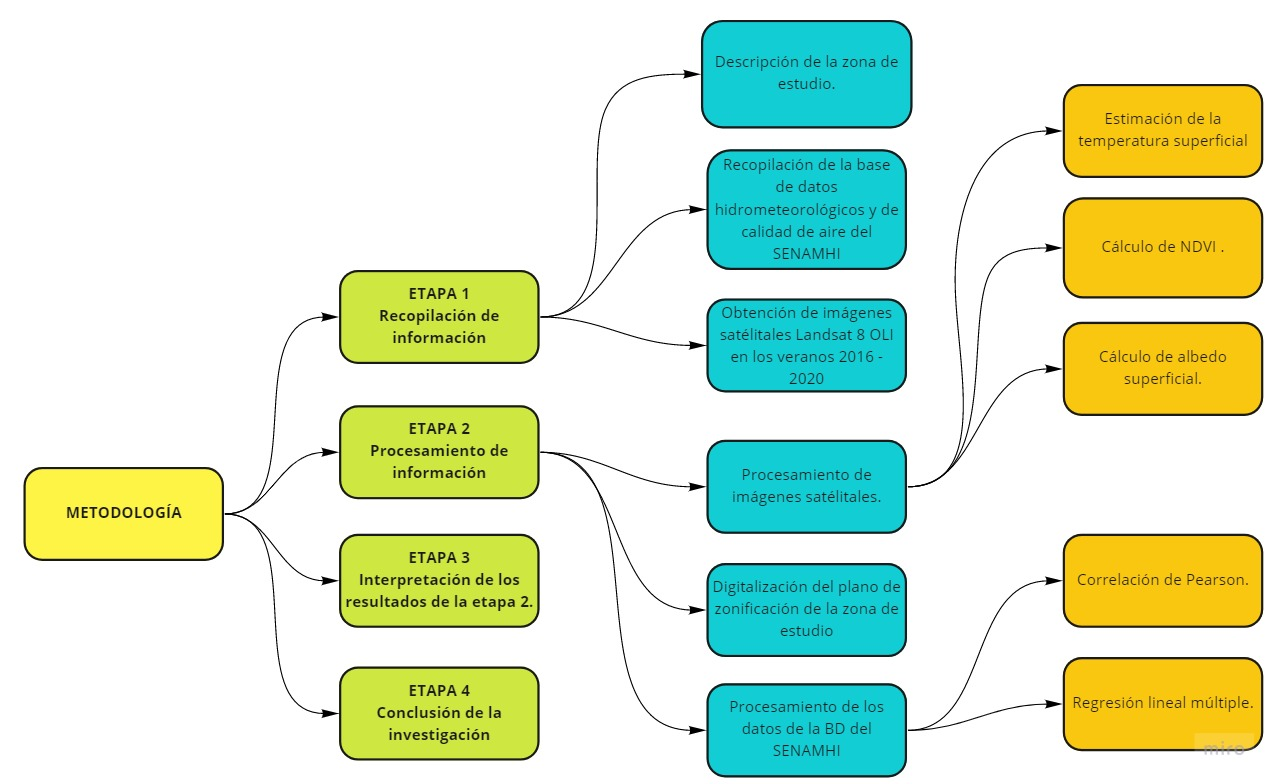
\includegraphics{Img/Metodologia} \end{center}

\hypertarget{recopilaciuxf3n-de-la-informaciuxf3n}{%
\subsubsection{5.1. Recopilación de la
información}\label{recopilaciuxf3n-de-la-informaciuxf3n}}

\hypertarget{descripciuxf3n-de-la-zona-de-estudio}{%
\paragraph{5.1.1. Descripción de la zona de
estudio}\label{descripciuxf3n-de-la-zona-de-estudio}}

En este apartado, produciremos información relevante dentro del distrito
de Jesús María, digitalizando el planeamiento urbanístico del distrito y
clasificándolo por sectores vecinales y por los tipos de áreas que
predominan. Según la Municipalidad de Jesús María se establecieron nueve
sectores vecinales para una mejor administración.

\begin{Shaded}
\begin{Highlighting}[]
\CommentTok{# Este es un mapa dinamico}

\CommentTok{# Datos}
\NormalTok{SuelosJM <-}\StringTok{ }\NormalTok{ee}\OperatorTok{$}\KeywordTok{FeatureCollection}\NormalTok{(}\StringTok{'users/juliocontreras1/JesusMSueloU'}\NormalTok{)}
\NormalTok{jm <-}\StringTok{ }\KeywordTok{ee_as_sf}\NormalTok{(SuelosJM) }\OperatorTok\StringTok{ }\KeywordTok{st_cast}\NormalTok{(}\StringTok{"MULTIPOLYGON"}\NormalTok{)}

\CommentTok{# Colores y variables necesarias para generar grupos}
\NormalTok{Number_JmType <-}\StringTok{ }\NormalTok{jm}\OperatorTok{$}\NormalTok{Type }\OperatorTok\StringTok{ }\KeywordTok{unique}\NormalTok{() }\OperatorTok\StringTok{ }\KeywordTok{length}\NormalTok{() }\CommentTok{# Numero de especies}
\NormalTok{Names_JmType <-}\StringTok{ }\NormalTok{jm}\OperatorTok{$}\NormalTok{Type }\OperatorTok\StringTok{ }\KeywordTok{unique}\NormalTok{() }\CommentTok{# Nombre de las especies}
\NormalTok{Colores <-}\StringTok{ }\KeywordTok{c}\NormalTok{(}\StringTok{"#ef3b2c"}\NormalTok{, }\StringTok{"#ffffff"}\NormalTok{, }\StringTok{"#807dba"}\NormalTok{, }\StringTok{"#33a02c"}\NormalTok{, }\StringTok{"#fed976"}\NormalTok{, }
             \StringTok{"#000000"}\NormalTok{, }\StringTok{"#0570b0"}\NormalTok{) }\CommentTok{# colorbrewer2, Colores de las especies seran}
\NormalTok{pal <-}\StringTok{ }\KeywordTok{colorFactor}\NormalTok{(Colores, }\DataTypeTok{domain =}\NormalTok{ Names_JmType) }\CommentTok{# Generamos la paleta}

\CommentTok{# Mapa SuelosU}
\KeywordTok{leaflet}\NormalTok{() }\OperatorTok\StringTok{ }
\StringTok{  }\KeywordTok{addTiles}\NormalTok{() }\OperatorTok\StringTok{ }
\StringTok{  }\KeywordTok{addPolygons}\NormalTok{(}\DataTypeTok{data =}\NormalTok{ jm,}
              \DataTypeTok{fillColor =} \OperatorTok{~}\KeywordTok{pal}\NormalTok{(Type),}
              \DataTypeTok{fillOpacity =} \FloatTok{0.8}\NormalTok{,}
              \DataTypeTok{weight =} \FloatTok{0.5}\NormalTok{,}
              \DataTypeTok{label =} \OperatorTok{~}\NormalTok{Type,}
              \DataTypeTok{color =} \StringTok{"#000000"}\NormalTok{,}
              \DataTypeTok{group =} \StringTok{"SuelosU"}\NormalTok{) }\OperatorTok
\StringTok{  }\KeywordTok{addLegend}\NormalTok{(}\DataTypeTok{data =}\NormalTok{ jm, }\StringTok{"bottomright"}\NormalTok{, }\DataTypeTok{pal =}\NormalTok{ pal, }
                \DataTypeTok{values =} \OperatorTok{~}\NormalTok{Type, }\DataTypeTok{title =} \StringTok{"Suelos Urbanos"}\NormalTok{, }
                \DataTypeTok{opacity =} \FloatTok{0.8}\NormalTok{, }\DataTypeTok{group =} \StringTok{"Leyenda"}\NormalTok{) }\OperatorTok\StringTok{ }
\StringTok{  }\KeywordTok{addLayersControl}\NormalTok{(}\DataTypeTok{overlayGroups =} \StringTok{"SuelosU"}\NormalTok{, }
                   \DataTypeTok{options =} \KeywordTok{layersControlOptions}\NormalTok{(}\DataTypeTok{collapsed =} \OtherTok{TRUE}\NormalTok{))}

\CommentTok{#%>% # Falta popup = ~colum la hacer clic}
\end{Highlighting}
\end{Shaded}

\begin{Shaded}
\begin{Highlighting}[]
\CommentTok{# Este es más dinámico}

\CommentTok{# Datos}
\CommentTok{# SuelosJM <- ee$FeatureCollection('users/juliocontreras1/JesusMSueloU')}
\CommentTok{# jm <- ee_as_sf(SuelosJM) %>% st_cast("MULTIPOLYGON")}

\NormalTok{Number_JmType <-}\StringTok{ }\NormalTok{jm}\OperatorTok{$}\NormalTok{Type }\OperatorTok\StringTok{ }\KeywordTok{unique}\NormalTok{() }\OperatorTok\StringTok{ }\KeywordTok{length}\NormalTok{() }\CommentTok{# Numero de especies}
\NormalTok{Names_JmType <-}\StringTok{ }\NormalTok{jm}\OperatorTok{$}\NormalTok{Type }\OperatorTok\StringTok{ }\KeywordTok{unique}\NormalTok{() }\CommentTok{## Nombre de las especies}
\NormalTok{Colores <-}\StringTok{ }\KeywordTok{c}\NormalTok{(}\StringTok{"#ef3b2c"}\NormalTok{, }\StringTok{"#ffffff"}\NormalTok{, }\StringTok{"#807dba"}\NormalTok{, }\StringTok{"#33a02c"}\NormalTok{, }\StringTok{"#fed976"}\NormalTok{, }
             \StringTok{"#000000"}\NormalTok{, }\StringTok{"#0570b0"}\NormalTok{) }\CommentTok{# colorbrewer2, Colores de las especies seran}
\NormalTok{pal <-}\StringTok{ }\KeywordTok{colorFactor}\NormalTok{(Colores, }\DataTypeTok{domain =}\NormalTok{ Names_JmType) }\CommentTok{# Generamos la paleta}


\CommentTok{# Partimos un sf en varios sf}
\NormalTok{Spp_Pres <-}\StringTok{ }\KeywordTok{list}\NormalTok{()}
\ControlFlowTok{for}\NormalTok{ (i }\ControlFlowTok{in} \DecValTok{1}\OperatorTok{:}\KeywordTok{length}\NormalTok{(Names_JmType)) \{}
\NormalTok{  Spp_Pres[[i]] <-}\StringTok{ }\NormalTok{jm }\OperatorTok\StringTok{ }\NormalTok{dplyr}\OperatorTok{::}\KeywordTok{filter}\NormalTok{(Type }\OperatorTok{==}\StringTok{ }\NormalTok{Names_JmType[i])}
\NormalTok{\}}
\KeywordTok{names}\NormalTok{(Spp_Pres) <-}\StringTok{ }\NormalTok{Names_JmType}

\CommentTok{# Ploteamos cada sf, pero sin leyenda}
\NormalTok{Spp_Map <-}\StringTok{ }\KeywordTok{leaflet}\NormalTok{() }\OperatorTok\StringTok{ }\KeywordTok{addTiles}\NormalTok{()}
\ControlFlowTok{for}\NormalTok{ (i }\ControlFlowTok{in} \DecValTok{1}\OperatorTok{:}\KeywordTok{length}\NormalTok{(Spp_Pres)) \{}
\NormalTok{  Spp_Map <-}\StringTok{ }\NormalTok{Spp_Map }\OperatorTok
\StringTok{    }\KeywordTok{addPolygons}\NormalTok{(}\DataTypeTok{data =}\NormalTok{ Spp_Pres[[i]],}
              \DataTypeTok{fillColor =} \OperatorTok{~}\KeywordTok{pal}\NormalTok{(Type),}
              \DataTypeTok{fillOpacity =} \FloatTok{0.8}\NormalTok{,}
              \DataTypeTok{weight =} \FloatTok{0.5}\NormalTok{,}
              \DataTypeTok{label =} \OperatorTok{~}\NormalTok{Type,}
              \DataTypeTok{color =} \StringTok{"#000000"}\NormalTok{,}
              \DataTypeTok{group =}\NormalTok{  Names_JmType[i])}
\NormalTok{\}}

\CommentTok{# Agremos leyenda y su visualizador por grupos, tanto leyenda como suelos}
\NormalTok{Spp_Map <-}\StringTok{ }\NormalTok{Spp_Map }\OperatorTok
\StringTok{  }\KeywordTok{addLegend}\NormalTok{(}\DataTypeTok{data =}\NormalTok{ jm, }\StringTok{"bottomright"}\NormalTok{, }\DataTypeTok{pal =}\NormalTok{ pal, }
                \DataTypeTok{values =} \OperatorTok{~}\NormalTok{Type, }\DataTypeTok{title =} \StringTok{"Suelos Urbanos"}\NormalTok{, }
                \DataTypeTok{opacity =} \FloatTok{0.8}\NormalTok{, }\DataTypeTok{group =} \StringTok{"Leyenda"}\NormalTok{) }\OperatorTok
\StringTok{  }\KeywordTok{addLayersControl}\NormalTok{(}\DataTypeTok{overlayGroups =} \KeywordTok{c}\NormalTok{(}\StringTok{"Leyenda"}\NormalTok{, Names_JmType),}
                                      \DataTypeTok{options =} \KeywordTok{layersControlOptions}\NormalTok{(}\DataTypeTok{collapsed =} \OtherTok{TRUE}\NormalTok{))}
\NormalTok{Spp_Map}
\end{Highlighting}
\end{Shaded}

\begin{center}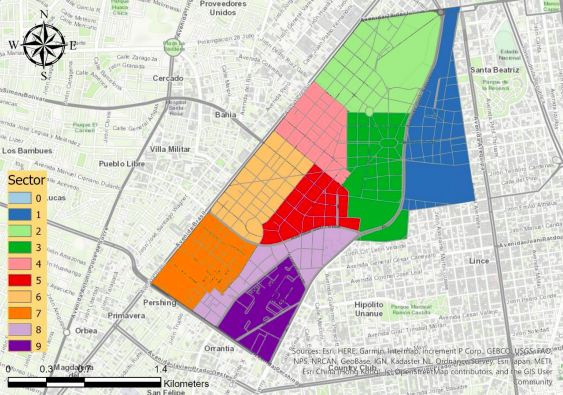
\includegraphics[width=7.82in]{Img/Sectores} \end{center}

\hypertarget{recopilaciuxf3n-de-la-base-de-datos-hidrometeoroluxf3gicos-y-de-calidad-del-aire-del-senamhi}{%
\paragraph{5.1.2. Recopilación de la base de datos hidrometeorológicos y
de calidad del aire del
SENAMHI}\label{recopilaciuxf3n-de-la-base-de-datos-hidrometeoroluxf3gicos-y-de-calidad-del-aire-del-senamhi}}

Las variables de temperatura, humedad relativa, precipitación, velocidad
del viento fueron extraídas del sitio web oficial de SENHAMI mediante
web scrapping en Python en las fechas disponibles desde 2015-05-01 hasta
la fecha actual.

La calidad del aire se calcula mediante variables atmosféricas como la
concentración de contaminación atmosférica: PM 2.5, PM10, O3, SO2, NO2
del sitio web oficial de SENHAMI en las fechas disponibles desde
2013-01-09 hasta la fecha actual.

\hypertarget{obtenciuxf3n-de-las-imuxe1genes-satuxe9litales-landsat-8-oli-en-los-veranos-2016-2020}{%
\paragraph{5.1.3. Obtención de las imágenes satélitales Landsat 8 OLI en
los veranos
2016-2020}\label{obtenciuxf3n-de-las-imuxe1genes-satuxe9litales-landsat-8-oli-en-los-veranos-2016-2020}}

Las imágenes satélites son proporcionadas por Landsat 8, estas son
imágenes extraídas sin nubes y recortadas en el distrito de Jesús María
a través de un script de Google Earth Engine filtrado en los meses de
verano de 2016 a 2020.

\hypertarget{procesamiento-de-la-informaciuxf3n}{%
\subsubsection{5.2. Procesamiento de la
información}\label{procesamiento-de-la-informaciuxf3n}}

\hypertarget{estimaciuxf3n-de-la-temperatura-de-superficie}{%
\paragraph{5.2.1. Estimación de la temperatura de
superficie}\label{estimaciuxf3n-de-la-temperatura-de-superficie}}

La temperatura de la superficie mide la emisión de radiación térmica de
la superficie terrestre donde la energía solar entrante interactúa y
calienta el suelo (Glynn C. Hulley, 2019).

Esta variable es una de las más importantes debido a que proporciona una
imagen más amplia de cómo se distribuye la temperatura en un área a
diferencia de la temperatura obtenida de las estaciones meteorológicas.

\hypertarget{landsat-dn-a-radiance}{%
\subparagraph{\texorpdfstring{\emph{Landsat DN a
Radiance}}{Landsat DN a Radiance}}\label{landsat-dn-a-radiance}}

Hay dos fórmulas que se pueden utilizar para convertir DN en
luminosidad; el método que utilice depende de los datos de calibración
de la escena disponibles en los archivos de encabezado. Un método
utiliza los valores de ganancia y sesgo (o compensación) del archivo de
encabezado. El otro método utiliza los factores de escala de radiancia
espectral LMin y LMax.

Aunque, el método utilizado en Landsat 8 OLI / TIRS es como el método de
ganancia y sesgo:

\[ L_{\lambda} = M_{\lambda} + Q_{cal} + A_{L}\]

Donde \(L_{\lambda}\) es un resplandor y \(M_{\lambda}\) y \(A_{L}\) son
Radiance Band Multiband y Add, respectivamente. La banda térmica
utilizada en el Landsat 8 es la número 10 con su correspondiente DN
\((𝑄_{cal})\). Estos datos se pueden encontrar en los metadatos de
Landsat 8.

\hypertarget{radiaciuxf3n-a-temperatura-de-brillo-en-grados-celsius}{%
\subparagraph{\texorpdfstring{\emph{Radiación a temperatura de brillo en
grados
Celsius}}{Radiación a temperatura de brillo en grados Celsius}}\label{radiaciuxf3n-a-temperatura-de-brillo-en-grados-celsius}}

\[ TB = \frac{K_{2}}{\ln([\frac{K_{1}}{L\lambda}])} - 273.15\]

Donde \(K_{1}\) y \(K_{2}\) representan la temperatura térmica
específica de la banda constantes de conversión de los metadatos y
\(L_{\lambda}\) es la banda de radiancia.

\hypertarget{temperatura-de-brillo-a-temperatura-de-superficie}{%
\subparagraph{\texorpdfstring{\emph{Temperatura de brillo a temperatura
de
superficie}}{Temperatura de brillo a temperatura de superficie}}\label{temperatura-de-brillo-a-temperatura-de-superficie}}

\[ S_{T^{°}} = \frac{TB}{1+\lambda+(\frac{TB}{\rho}) * \ln(\varepsilon)} \]

Donde \(TB\) es una temperatura de brillo, \(\lambda\) es la longitud de
onda de la radiancia emitida, \(\rho\) es una constante calculada por
esta ecuación:

\[ \rho = \frac{h *c}{\sigma} \]

Eso da como resultado \(1.4388 × 10^{-2} m K\) o \(14388 \mu m K\),
donde 𝜎 es la constante de Boltzmann \((1.38 × 10^{−23} J / K)\), \(h\)
es la constante de Planck \((6.626 × 10^{−34} \ J s)\) y \(c\) es la
velocidad de luz \((2.998 × 10^{8} \frac{m}{s})\). Y \(\varepsilon\) es
la emisividad de la superficie, que se explicará pronto.

\hypertarget{uxedndice-de-vegetaciuxf3n-de-diferencia-normalizada}{%
\paragraph{5.2.2. Índice de vegetación de diferencia
normalizada}\label{uxedndice-de-vegetaciuxf3n-de-diferencia-normalizada}}

Cuantifica la vegetación, su vigor y calidad, midiendo la diferencia
entre el infrarrojo cercano (que la vegetación refleja fuertemente) y la
luz roja (que la vegetación absorbe). Usamos bandas infrarrojas y rojas
para calcular el NDVI.

\[ NDVI = \frac{NIR_{b5}-RED_{b4}}{NIR_{b5}+RED_{b4}}\]

\hypertarget{emisividad-superficial}{%
\subparagraph{\texorpdfstring{\emph{Emisividad
superficial}}{Emisividad superficial}}\label{emisividad-superficial}}

Es un factor de proporcionalidad que escala el resplandor del cuerpo
negro (ley de Planck) para predecir el resplandor emitido, y es la
eficiencia de transmitir energía térmica a través de la superficie hacia
la atmósfera (Jovanovska, 2016).

Para calcular la emisividad de la superficie (\(\varepsilon\)) es
importante comprender cómo funciona y cómo se relaciona con el NDVI:

\[NDVI < 0, \hspace{4em} \varepsilon = 0.991\]
\[0 \le NDVI \le 0.2, \hspace{4em} \varepsilon = 0.996\]
\[0.2 \le NDVI \le 0.5, \hspace{4em} \varepsilon = 0.996 + 0.004 + P_{v}\]
\[0.2 < NDVI, \hspace{4em} \varepsilon = 0.973\] Donde \(P_{v}\) es la
fracción de cobertura de vegetación que equivale a:

\[ P_{v} = (\frac{NDVI-NDVI_{MIN \ VALUE}}{NDVI_{MAX \ VALUE} -NDVI_{MIN \ VALUE}})^2\]

\hypertarget{cuxe1lculo-del-albedo-superficial}{%
\paragraph{5.2.3. Cálculo del albedo
superficial}\label{cuxe1lculo-del-albedo-superficial}}

El albedo de superficie se define como la relación entre la radiosidad y
la irradiancia (flujo por unidad de área) que recibe una superficie. La
proporción reflejada no solo está determinada por las propiedades de la
propia superficie, sino también por la distribución espectral y angular
de la radiación solar que llega a la superficie de la Tierra (Coakley,
2003).

En este sentido, para la estimación de este parámetro se realizaron una
serie de algoritmos para calcular el albedo de varios sensores
satelitales con Landsat, donde la regresión lineal múltiple de mejor
ajuste fue descrita y normalizada por Smith en 2010.

\hypertarget{radiancia-a-reflectancia-toa}{%
\subparagraph{\texorpdfstring{\emph{Radiancia a reflectancia
TOA}}{Radiancia a reflectancia TOA}}\label{radiancia-a-reflectancia-toa}}

Para Landsat 8

\[ \rho_{\lambda^{'}} = M_{p} + Q_{cal} + A_{p} \]

Donde \(\rho_{\lambda^{'}}\) es reflectancia sin corrección del ángulo
solar y \(M_{p}\) y \(A_{p}\) son bandas de reflectancia multibanda y
\textbf{Add}, respectivamente. Las bandas utilizadas en el Landsat 8 son
los números \(1,3,4,5,7\) con su correspondiente DN \((Q_{cal})\). Esto
Los datos se pueden encontrar en los metadatos de Landsat 8.

Para corregir esta reflectancia para cada banda, usaremos esta ecuación:

\[\rho_{\lambda} = \frac{\rho_{\lambda^{'}}}{\cos{\theta_{sz}}}\] Donde:
* \(\rho_{\lambda}\) es la reflectancia calculada con el ángulo
corrección para cada banda \(1,3,4,5,7\). * \(\theta_{sz}\) (ángulo
cenital) es igual a 90 - ángulo de elevación del sol = 35.09 (en este
caso)

\hypertarget{bandas-de-reflectancia-al-albedo-de-superficie}{%
\subparagraph{\texorpdfstring{\emph{Bandas de reflectancia al albedo de
superficie}}{Bandas de reflectancia al albedo de superficie}}\label{bandas-de-reflectancia-al-albedo-de-superficie}}

Una vez que haya llegado el momento de obtener la reflectancia, puede
utilizar la fórmula que desarrolló. Su fórmula Landsat para calcular el
albedo de superficie de onda corta.

\[\alpha = 0.356 + \rho_{\lambda_{1}} + 0.130 * \rho_{\lambda_{2}} + 0.085 +\rho_{\lambda_{5}} + 0.072 * \rho_{\lambda_{7}}\]

\hypertarget{digitalizaciuxf3n-del-plano-de-zonificaciuxf3n}{%
\subsubsection{5.3. Digitalización del plano de
zonificación}\label{digitalizaciuxf3n-del-plano-de-zonificaciuxf3n}}

Según el Instituto Metropolitano de Planificación en el Reajuste
Integral de la zonificación de usos del suelo en Lima Metropolitana se
dividió el distrito de Jesús María en seis áreas principales.

\begin{center}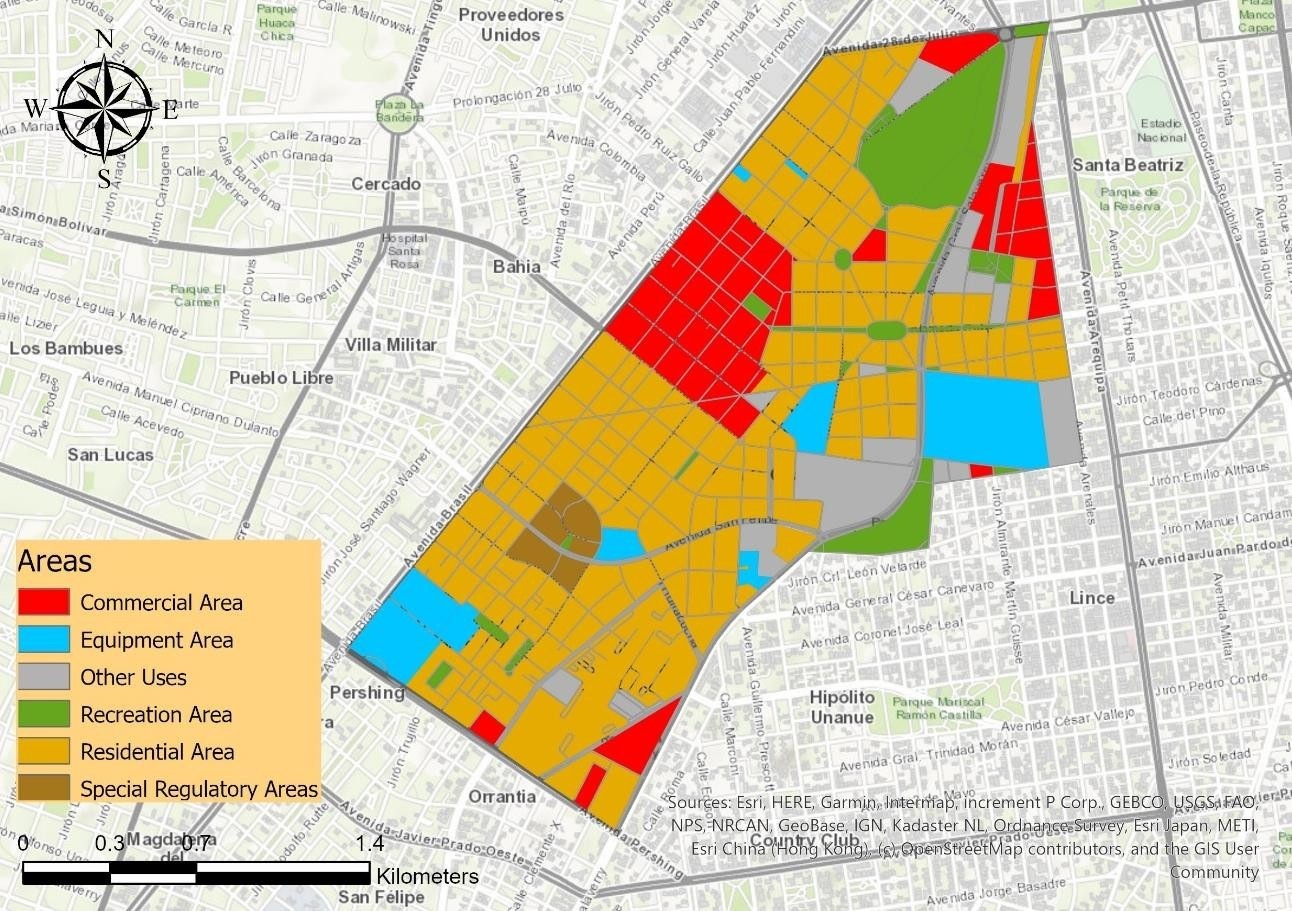
\includegraphics{Img/distrito_clasificado} \end{center}

\begin{itemize}
\tightlist
\item
  \textbf{Área comercial:} Son las áreas urbanas destinadas
  principalmente a la ubicación y operación de establecimientos para la
  compra - venta de productos y servicios.
\item
  \textbf{Área de edificación:} Se refiere a las áreas urbanas
  destinadas a brindar servicios primarios como salud y educación. Los
  centros de salud, hospitales y escuelas se clasifican en esta área.
\item
  \textbf{Área de otros usos:} ¿Son áreas urbanas destinadas
  principalmente a la habilitación y funcionamiento de instalaciones con
  fines especiales como museos, municipios, embajadas, oficinas
  centrales, etc.
\item
  \textbf{Área de recreación:} Áreas que se encuentran en áreas urbanas
  o de expansión urbana destinadas principalmente a la realización de
  actividades recreativas activas y / o pasivas, tales como: Plazas,
  Parques, piscinas de agua, áreas verdes, y similares.
\item
  \textbf{Barrio residencial:} Son áreas urbanas destinadas
  predominantemente al uso de vivienda y también pueden tolerar otros
  usos compatibles. Los planes de zonificación incluyen: Zona de alta
  densidad (RDA), Zona de densidad media (RDM) y Zona de baja densidad
  (RDB).
\item
  \textbf{Área reguladora especial:} El propósito de las áreas urbanas
  se basa en la mejora urbana: descongestión, creación de dotaciones,
  saneamiento, problemas de circulación y otros problemas similares.
\end{itemize}

\hypertarget{procesamiento-de-los-datos-de-la-bd-del-senmahi}{%
\subsubsection{5.4.Procesamiento de los datos de la BD del
SENMAHI}\label{procesamiento-de-los-datos-de-la-bd-del-senmahi}}

Los datos del modelo calculado y los datos extraídos están en diferentes
esquemas y disponibles en diferentes fechas. Para ello, fusionaremos los
datos en común y se eliminarán los datos no disponibles.

En esta sección exploraremos las variables hidrometeorológicas y de
contaminación del aire disponibles en la fecha de verano de esta
estación.

Imagenes a pegar\ldots{}

\hypertarget{resultados}{%
\subsection{6. Resultados}\label{resultados}}

\hypertarget{identificaciuxf3n-de-la-isla-de-calor-urbana}{%
\subsubsection{6.1 Identificación de la isla de calor
urbana}\label{identificaciuxf3n-de-la-isla-de-calor-urbana}}

Cabe señalar que los datos calculados a partir del modelo son el
resultado de la media de las imágenes de satélite por verano, es decir,
para identificar las islas de calor urbanas, la temperatura debe ser
superior a la media y en su entorno.

\begin{longtable}[]{@{}llll@{}}
\toprule
VERANO & ST MIN (° C) & ST MAX (° C) & ST PROMEDIO (° C)\tabularnewline
\midrule
\endhead
2016 & 21.58 & 26,7 & 23,95\tabularnewline
2017 & 26,89 & 34,45 & 30,42\tabularnewline
2018 & 21.16 & 28.09 & 24,88\tabularnewline
2019 & 23.52 & 28,91 & 26,32\tabularnewline
2020 & 23,87 & 29,32 & 26,6\tabularnewline
\bottomrule
\end{longtable}

\begin{center}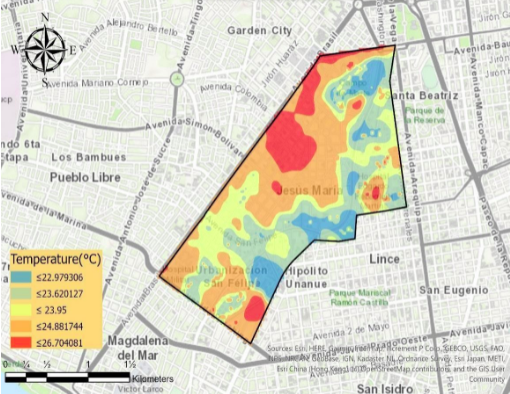
\includegraphics[width=7.08in]{Img/Islas} \end{center}

Y otras islas calor\ldots{}

\hypertarget{interpretaciuxf3n-los-resultados-de-los-datos-calculados}{%
\subsubsection{6.2 Interpretación los resultados de los datos
calculados}\label{interpretaciuxf3n-los-resultados-de-los-datos-calculados}}

\begin{enumerate}
\def\labelenumi{\alph{enumi})}
\tightlist
\item
  El NDVI es mayor en áreas de recreación por tener áreas verdes y menor
  en áreas comerciales, así mismo los equipos y áreas residenciales
  tienen valores promedio bajos debido a su escasa o nula vegetación.
\end{enumerate}

\begin{center}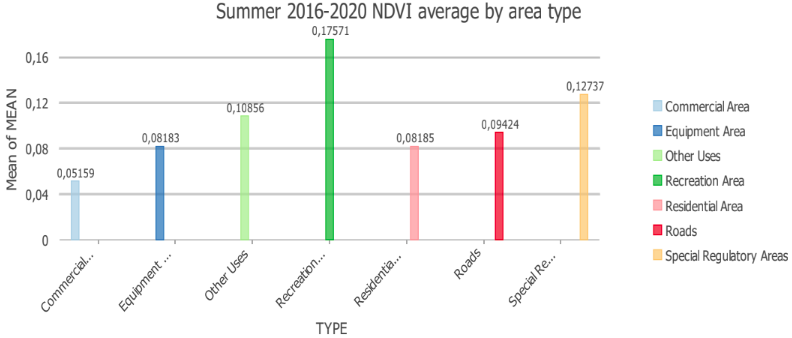
\includegraphics[width=0.8\linewidth]{Img/interpretacionislas} \end{center}

\begin{enumerate}
\def\labelenumi{\alph{enumi})}
\setcounter{enumi}{1}
\item
  Todas estas áreas tienen un albedo similar y con poca variación, el
  los promedios más altos de albedo son del equipo y especial áreas
  regulatorias, principalmente porque están pintadas en colores claros
  que reflejan el calor incidente. Por otro lado, las áreas de
  recreación y las calles construidas con asfalto tienen valores de
  albedo más bajos.
\item
  En el caso de la temperatura superficial, las áreas con alta
  temperatura valor son el área comercial y de equipos que superan
  fácilmente el promedio de cada verano, junto con áreas de Otros Usos y
  áreas cercanas para ellos, las zonas residenciales son las principales
  islas de calor urbanas.
\end{enumerate}

\hypertarget{anuxe1lisis}{%
\subsection{7. Análisis}\label{anuxe1lisis}}

\hypertarget{correlaciuxf3n-de-pearson-de-variables-calculadas}{%
\subsubsection{7.1 Correlación de Pearson de variables
calculadas}\label{correlaciuxf3n-de-pearson-de-variables-calculadas}}

\hypertarget{verano-2016}{%
\paragraph{\texorpdfstring{\emph{Verano
2016}}{Verano 2016}}\label{verano-2016}}

Se observa una fuerte correlación negativa del \(NDVI\) con la
temperatura superficial, lo que significa que con menor presencia de
vegetación, la temperatura aumenta. Además, el albedo superficial tiene
una correlación positiva moderada, por lo que la temperatura podría
aumentar con el albedo superficial.

\begin{longtable}[]{@{}cccc@{}}
\toprule
° & ST & ALBEDO & NDVI\tabularnewline
\midrule
\endhead
\textbf{ST} & 21.58 & 26,7 & 23,95\tabularnewline
\textbf{ALBEDO} & 26,89 & 34,45 & 30,42\tabularnewline
\textbf{NDVI} & 21.16 & 28.09 & 24,88\tabularnewline
\bottomrule
\end{longtable}

\hypertarget{verano-2017}{%
\paragraph{\texorpdfstring{\emph{Verano
2017}}{Verano 2017}}\label{verano-2017}}

Es observadouna fuerte correlación negativa del NDVI con la temperatura
superficial, lo que significa que con menor presencia de vegetación, la
temperatura aumenta. Además, el albedo superficial tiene una correlación
negativa débil, por lo que la temperatura no podría verse afectada por
el albedo en este verano.

\hypertarget{verano-2018}{%
\paragraph{\texorpdfstring{\emph{Verano
2018}}{Verano 2018}}\label{verano-2018}}

Se observa una correlación negativa moderada del NDVI con la temperatura
superficial, lo que significa que con menor presencia de vegetación, la
temperatura podría aumentar. Además, el albedo de la superficie tiene
una correlación negativa débil, por lo que la temperatura podría no
verse tan afectada por el albedo en este verano

\hypertarget{verano-2019}{%
\paragraph{\texorpdfstring{\emph{Verano
2019}}{Verano 2019}}\label{verano-2019}}

Es observadouna fuerte correlación negativa del NDVI con la temperatura
superficial, lo que significa que con menor presencia de vegetación, la
temperatura aumenta. Además, el albedo de la superficie tiene una
correlación positiva débil, por lo que la temperatura podría no verse
tan afectada por el albedo en este verano.

\hypertarget{verano-2020}{%
\paragraph{\texorpdfstring{\emph{Verano
2020}}{Verano 2020}}\label{verano-2020}}

Es observadouna fuerte correlación negativa del NDVI con la temperatura
superficial, lo que significa que con menor presencia de vegetación, la
temperatura aumenta. Además, el albedo de la superficie tiene una
correlación positiva débil, por lo que la temperatura podría no verse
tan afectada por el albedo en este verano.

\hypertarget{resumen-de-resultados}{%
\paragraph{\texorpdfstring{\emph{Resumen de
Resultados}}{Resumen de Resultados}}\label{resumen-de-resultados}}

En la mayoría de los casos el NDVI tiene una correlación negativa
moderada o fuerte con la Temperatura de la Superficie, así mismo el
albedo de la superficie tiene una gran variación teniendo una
correlación moderada o débil y positiva o negativa, por lo que es una
variable no tan significativa al evaluar la temperatura de la
superficie. . Finalmente, el NDVI y el albedo superficial siempre han
tenido una fuerte correlación negativa en los últimos cinco veranos.

\hypertarget{correlaciuxf3n-de-variables}{%
\subsubsection{7.3 Correlación de
variables}\label{correlaciuxf3n-de-variables}}

En la tabla que se muestra a continuación podemos relacionar las
variables calculadas, en el píxel donde se ubica la estación, con la
temperatura obtenida de la estación meteorológica. Podemos ver que
existe una fuerte correlación positiva entre la temperatura obtenida de
la estación con la temperatura superficial, así mismo la disminución del
albedo traerá un aumento en ambas temperaturas y por último al estar la
estación en una zona verde el NDVI no disminuirá con tiempo
extraordinario.

Tabla de correlación\ldots{}

\hypertarget{regresiuxf3n-lineal-de-variables-hidrometeoroluxf3gicas-y-de-calidad-ambiental}{%
\subsubsection{7.4. Regresión lineal de variables hidrometeorológicas y
de calidad
ambiental}\label{regresiuxf3n-lineal-de-variables-hidrometeoroluxf3gicas-y-de-calidad-ambiental}}

Con los datos extraídos disponibles, realizamos una regresión lineal
múltiple para visualizar la influencia de las variables sobre la
temperatura. Los resultados fueron los siguientes:

\[ T°_{2016}= 33.6102 + 0.0007 × PM_{10} + 0.0144 × O_{3} + 0.008 × NO_{2} + 0.6376 × CO - 1.1466 × Precipitation - 0.1415 × Humidity + 0.3609 × WindSpeed\]
Y las otras regresiones\ldots{}

\hypertarget{interpretaciuxf3n-de-resultados}{%
\paragraph{\texorpdfstring{\emph{Interpretación de
resultados}}{Interpretación de resultados}}\label{interpretaciuxf3n-de-resultados}}

Primero, llegamos a la conclusión de que hay una adición de temperatura
por los contaminantes del aire, a excepción de \(PM_{2.5}\), que ha ido
disminuyendo cada verano. En segundo lugar, con las variables
hidrometeorológicas: la precipitación, siendo casi nula y con pocos
datos, tiene coeficientes altos, pero en teoría no puede contribuir a la
temperatura. En cuanto a la humedad relativa disminuye con el aumento de
temperatura y finalmente la velocidad del viento ha aumentado con la
temperatura debido al calor es lo que mueve las masas de aire.

\hypertarget{discusiuxf3n-de-resultados}{%
\subsection{8. Discusión de
resultados}\label{discusiuxf3n-de-resultados}}

El principal problema del proyecto es la falta de información referente
a la base de datos del SENHAMI, por lo que se ajustó a las fechas
establecidas de verano durante cinco años, así mismo las colecciones de
imágenes satelitales solo se pudieron obtener en los meses de verano ya
que es donde se la resolución más alta.

\hypertarget{conclusiuxf3n}{%
\subsection{9. Conclusión}\label{conclusiuxf3n}}

En resumen, en conclusión se identificaron las islas de calor urbano
presentes principalmente en el ámbito comercial, de equipamiento, otros
usos y áreas residenciales cercanas a las mismas.

El NDVI tiene una fuerte correlación negativa con la temperatura
superficial y el Albedo superficial no presenta una gran correlación,
mientras que con la temperatura obtenida de la estación meteorológica
Campo de Marte tiene una buena correlación positiva con la temperatura
superficial, así mismo el albedo superficial disminuye con el aumento de
las temperaturas de la estación. En el caso de variables
hidrometeorológicas: La precipitación, siendo casi nula y con pocos
datos, tiene altos coeficientes, pero en teoría no puede contribuir a la
temperatura. En cuanto a la humedad relativa, disminuye con aumentando
la temperatura y finalmente la velocidad del viento ha aumentado con la
temperatura debido al calor es lo que mueve las masas de aire. Por
último, hay una adición de temperatura por los contaminantes del aire, a
excepción de \(PM_{2.5}\), que ha ido disminuyendo cada verano.

\hypertarget{referencias}{%
\subsection{10. Referencias}\label{referencias}}

oakley, JA (2003). REFLEXIÓN Y ALBEDO, SUPERFICIE. Prensa académica, 10.
FIQUITIVA, TZ (2017). ANÁLISIS ESPACIO-TEMPORAL DE VARIABLES QUE INCIDEN
EN LA GENERACIÓN DE ISLA DE CALOR URBANA EN LA LOCALIDAD DE KENNEDY.
UNIVERSIDAD SANTO TOMAS, SEDE BOGOTÁ.

Glynn C. Hulley, director general (2019). Tomando la temperatura de la
tierra. Elsevier. Jovanovska, UA (2016). Algoritmo para el mapeo
automatizado de la superficie terrestre Temperatura. Hindawi corporación
editorial.

Párraga, VS (2015). IDENTIFICACIÓN DE ISLAS DE CALOR EN LA CIUDAD DE
METROPOLITAN LIMA USANDO IMÁGENES SATELITALES 5TM. Universidad Nacional
Agraria La Molina, Lima - Perú.

Smith, R. (2010). ``El balance de calor de la superficie terrestre
deducido del espacio''.

\end{document}
